\section{Càlcul del primer esglaó del compressor}
Per tal de fer el càlcul del primer esglaó es consideraran diversos valors típics de solidesa i de flux. Amb aquests valors es calcularan els paràmetres necessaris per obtenir el rendiment i el treball per esglaó per a tots els casos. Un cop es tinguin aquests valors, es calcularà el treball necessari per esglaó considerant el treball total a assolir i el número més típic d'esglaons en compressors, trobant així una solució possible i òptima. 
Els valors de solidesa i flux que s'han considerat son:

\begin{equation}
\nonumber \frac{1}{\sigma}=[0.4; 0.6; 0.8; 1.0; 1.2]
\end{equation}
 
\begin{equation}
\nonumber \Psi=[0.4;0.5;0.6;0.7;0.8]
\end{equation}
\subsection{Càlcul de $\beta_a$ i $\beta_b$ en funció de $S/C$ i $\Psi$}
Per a calcular els angles que forma la corrent del flux amb l'eix del rotor, s'utilitzarà el criteri experimental de \textit{Howell} i les hipòtesis mencionades a l'apartat \ref{Intro}. S'obtenen tres equacions amb tres incògnites: $\beta_a$, $\beta_b$ i $\beta_m$: 
\begin{equation}
\tan(\beta_a)-\tan(\beta_b)=\frac{1.55}{1+1.55\frac{S}{C}}
\end{equation} 
\begin{equation}
\tan(\beta_m)=\frac{\tan(\beta_a)+\tan(\beta_b)}{2}
\end{equation}
\begin{equation}
\tan(\beta_m)=\frac{1}{2\Psi}
\end{equation}
Les incògnites es poden aïllar fàcilment per a poder resoldre el sistema. En les següents figures es mostren els resultats per a $\beta_a$ i $\beta_b$. $beta_m$ serà utilitzada per a càlculs posteriors.
\begin{figure}[H]
	\centering
	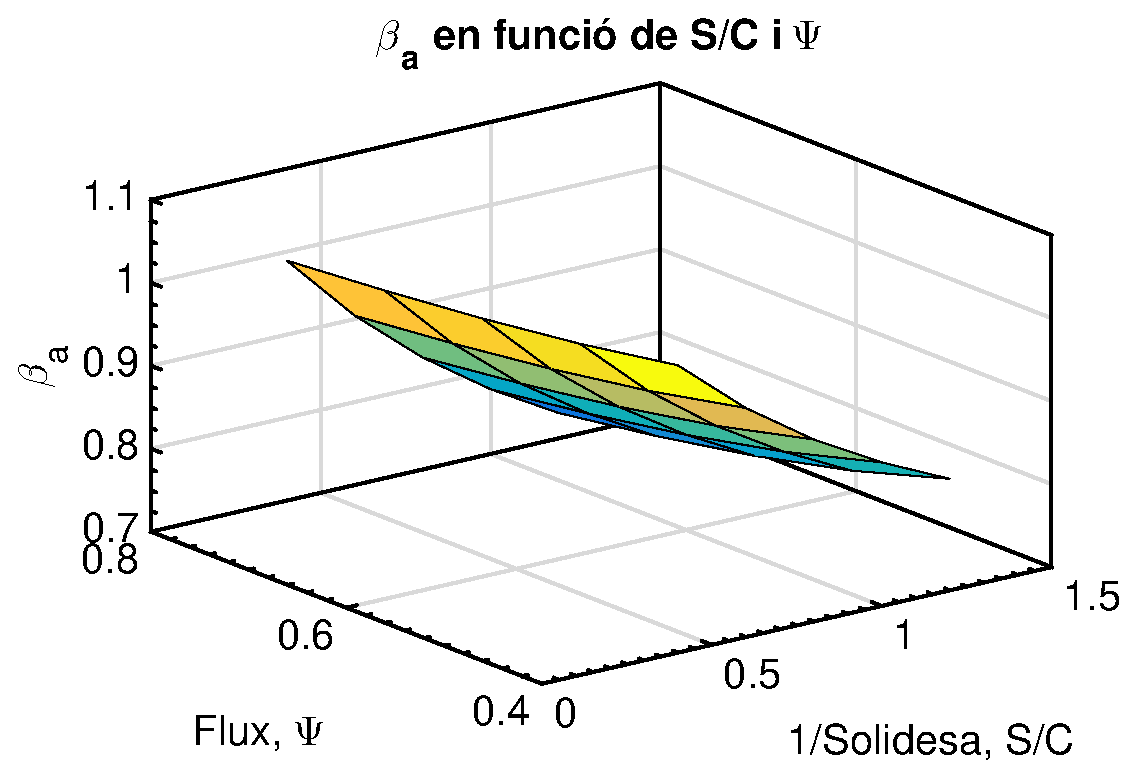
\includegraphics[width=0.8\textwidth]{./code/figures/parametres/betA}
	\caption{Valors de $\beta_a$ en funció de $S/C$ i $\Psi$.}
	\label{betA}
\end{figure}

\begin{figure}[H]
	\centering
	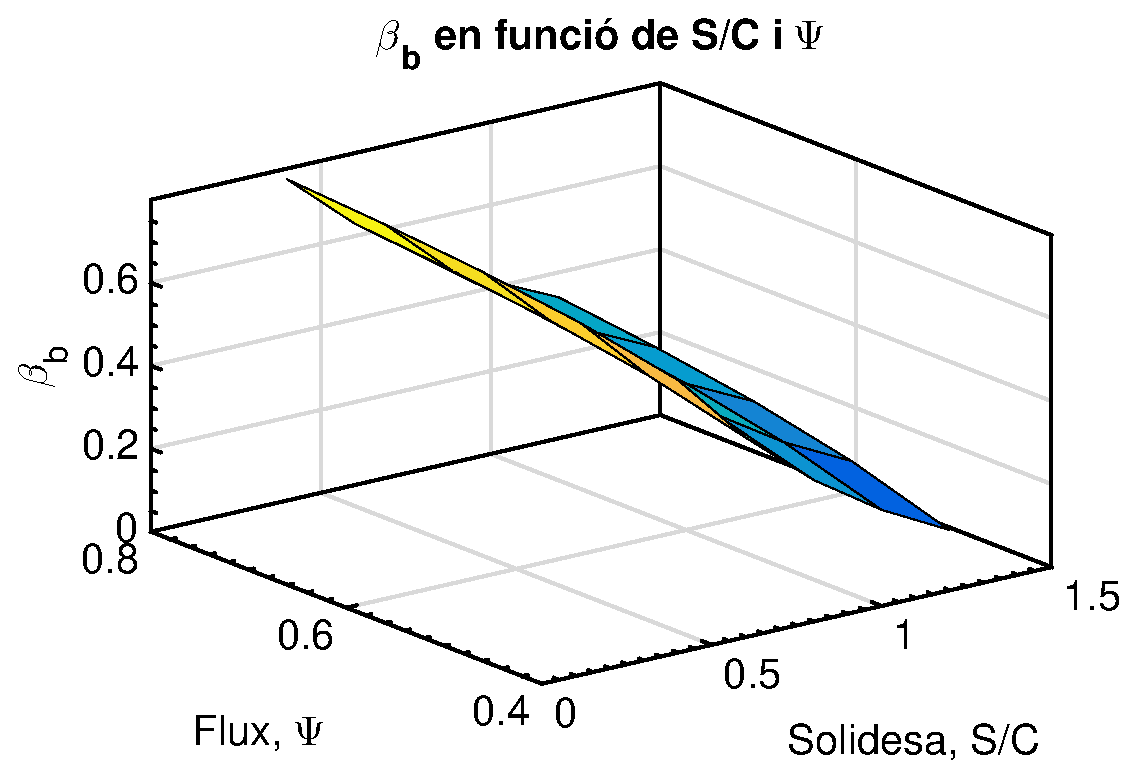
\includegraphics[width=0.8\textwidth]{./code/figures/parametres/betB}
	\caption{Valors de $\beta_b$ en funció de $S/C$ i $\Psi$.}
	\label{betB}
\end{figure}

\subsection{Càlcul de $C_D$ i $C_L$ en funció de $S/C$ i $\Psi$}
Les expressions per a calcular la sustentació i la resistència han sigut obtingudes analitzant el volum de control enter dos àleps. Se suposa que el procés que té lloc es estacionari i que el flux es incompressible. Es realitza un anàlisi utilitzant les equacions de la quantitat de moviment per obtenir la força en la direcció axial i en la direcció angular. A partir d'aquestes equacions, la sustentació i la resistència es poden calcular com: 
\begin{equation}
L= F_\theta \cos\beta_m+F_z \sin\beta_m
\end{equation}
\begin{equation}
D= F_\theta \sin\beta_m-F_z \cos\beta_m
\end{equation}
Substituint expressions i adimensionalitzant s'obté: 
\begin{equation}
C_L=2\frac{S}{C}(\tan\beta_a-\tan\beta_b)\cos\beta_m-C_D\tan\beta_m
\end{equation} 
\begin{equation}
C_D=0.021+\frac{0.02}{2.5}\frac{S}{C}+0.018C_L^2
\end{equation}
Que es un sistema de dues equacions amb dues incògnites. Els resultats es mostren en les següents figures.

\begin{figure}[H]
	\centering
	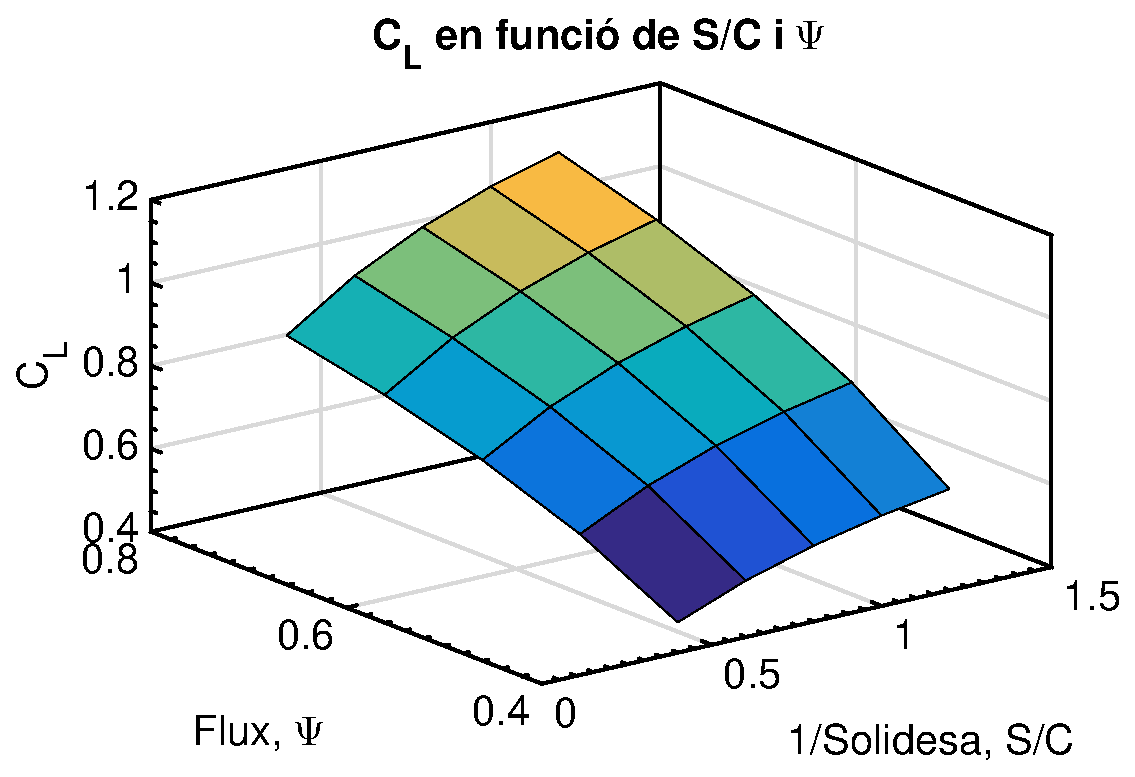
\includegraphics[width=0.8\textwidth]{./code/figures/parametres/CL}
	\caption{Valors de $C_L$ en funció de $S/C$ i $\Psi$.}
	\label{CL}
\end{figure}


\begin{figure}[H]
	\centering
	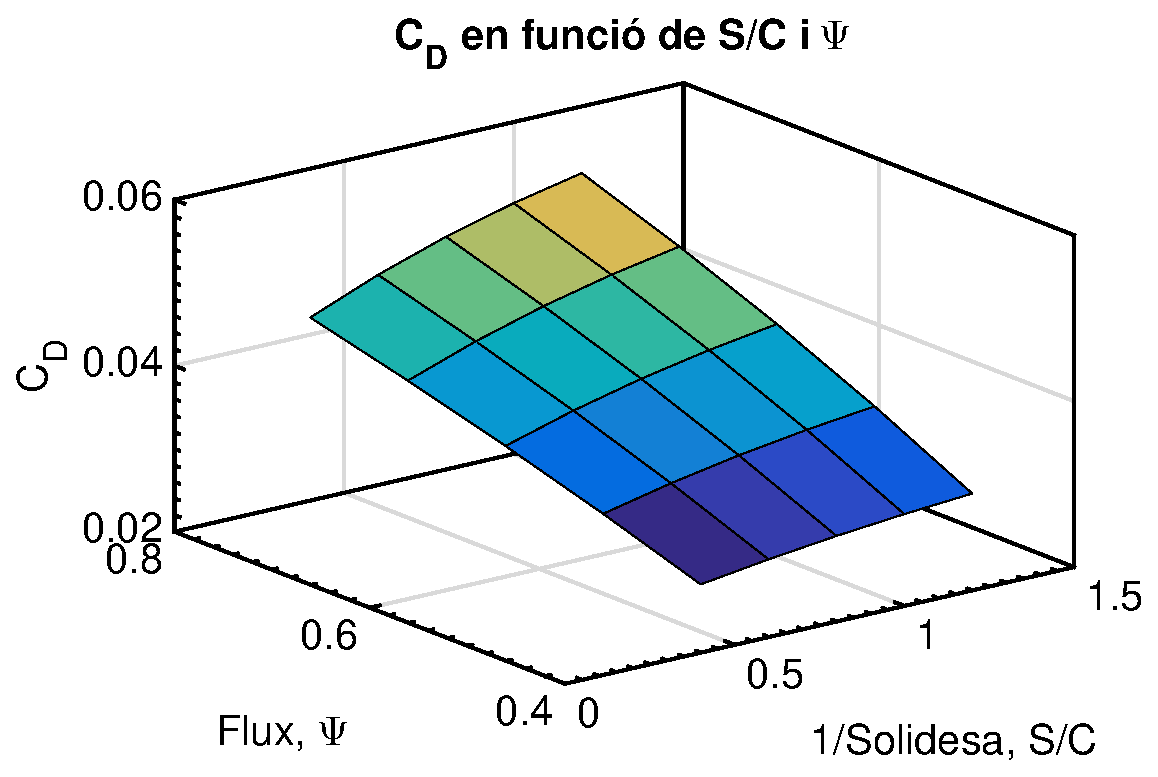
\includegraphics[width=0.8\textwidth]{./code/figures/parametres/CD}
	\caption{Valors de $C_D$ en funció de $S/C$ i $\Psi$.}
	\label{CD}
\end{figure}


\subsection{Càlcul del rendiment de l'esglaó en funció de $S/C$ i $\Psi$}
Els objectius que busquem son: 
\begin{itemize}
\item Mínim nombre d'esglaons possibles per tal de disminuir el pes i volum del compressor.
\item Rendiment adiabàtic bo.
\item Menor àrea frontal possible.
\end{itemize}
Es defineix el rendiment com:
\begin{equation}
\eta_{esg}=\frac{T_{ct}'-T_{0t}}{T_{ct}-T_{0t}}
\end{equation}
On $T_{ct}'$ es la temperatura a la sortida de l'etapa del compressor ideal i $T_{ct}$ la real. Aquest rendiment es pot re-escriure com:
\begin{equation}
\eta_{esg}=1-\frac{T_{it}-T_{bt}'}{T_{ct}-T_{0t}}-\frac{T_{bt}'-T_{ct}'}{T_{ct}-T_{0t}}
\end{equation}
Es a dir, a 1 se li resten les pèrdues del rotor i les pèrdues de l'estator. Relacionant les temperatures amb pressions mitjançant el coeficient $\gamma$:
\begin{equation}
\eta_{esg}=\frac{\bigtriangleup P_{r}+\bigtriangleup P_{e}}{\rho\tau_{esg}}
\end{equation}
Considerant que el grau de reacció es 0.5, la variació de pressió al rotor i a l'estator es la mateixa i per tant: 
\begin{equation}
\eta_{esg}=\frac{\bigtriangleup P_t}{\rho\tau_{esg}}
\end{equation}
Considerant les següents equacions: 
\begin{equation}
\bigtriangleup P_t=\frac{C_D\frac{1}{2}\rho\omega_m^2}{\frac{S}{C}\cos\beta_m}
\end{equation}
\begin{equation}
\tau_{esg}=U(V_{\theta_b}-V_{\theta_a})
\end{equation}
\begin{equation}
R=0.5=\Psi\tan\beta_m
\end{equation}
S'arriba a les següents expressions per al calcul del rendiment: 
\begin{equation}
\tau_{esg}=1-\frac{C_D}{C_{Li}}\Big( 2\Psi+\frac{1}{2\Psi}\Big)
\end{equation}
\begin{equation}
\tau_{23}=1-N\frac{C_D}{C_{Li}}\Big( 2\Psi+\frac{1}{2\Psi}\Big)
\end{equation}
Essent $N$ el nombre d'esglaons del compressor. $C_{Li}$ s'ha definit com: 
\begin{equation}
C_{Li}=\frac{2}{\sigma}(\tan\beta_a-\tan\beta_b)\cos\beta_m
\end{equation}
Finalment, el rendiment per esglaó es pot apreciar a la Figura \ref{ETAesg}. El rendiment total es podrà calcular un cop s'obtingui el nombre d'esglaons que tindrà el compressor. 
\begin{figure}[H]
	\centering
	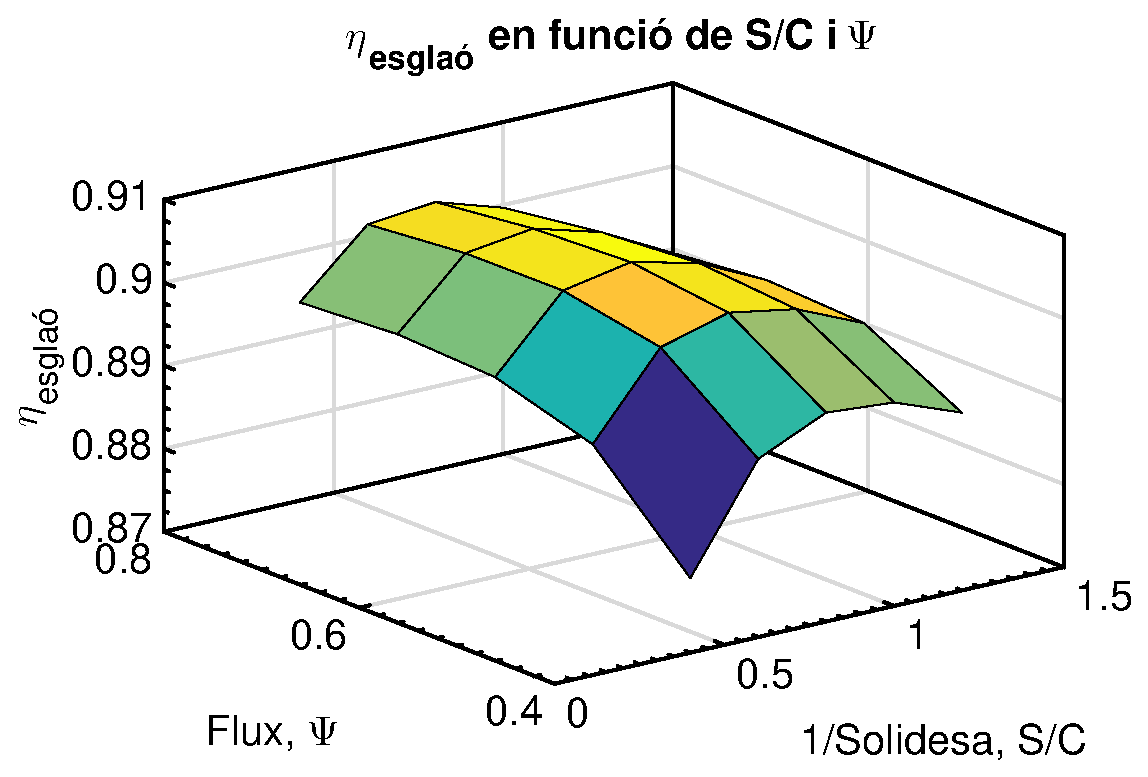
\includegraphics[width=0.8\textwidth]{./code/figures/parametres/ETAesg}
	\caption{Valors de $\eta_{esg}$ en funció de $S/C$ i $\Psi$.}
	\label{ETAesg}
\end{figure}

\subsection{Velocitat axial en funció de $S/C$ i $\Psi$}
La velocitat axial presenta una limitació en el disseny del compressor, ja que no interessa que hagi flux sònic a cap punt del perfil evitant així efectes de compressibilitat. Amb l'objectiu d'evitar aquest fenomen, es limita el número a 0.8. La velocitat axial es troba utilitzant la següent expressió: 
\begin{equation}
V_z=\sqrt{\frac{M^2\gamma R T_{at}}{\frac{1}{(\cos\beta_a)^2}+\frac{M^2\gamma R}{2C_P(\cos\beta_b)^2}}}
\end{equation} 
\begin{figure}[H]
	\centering
	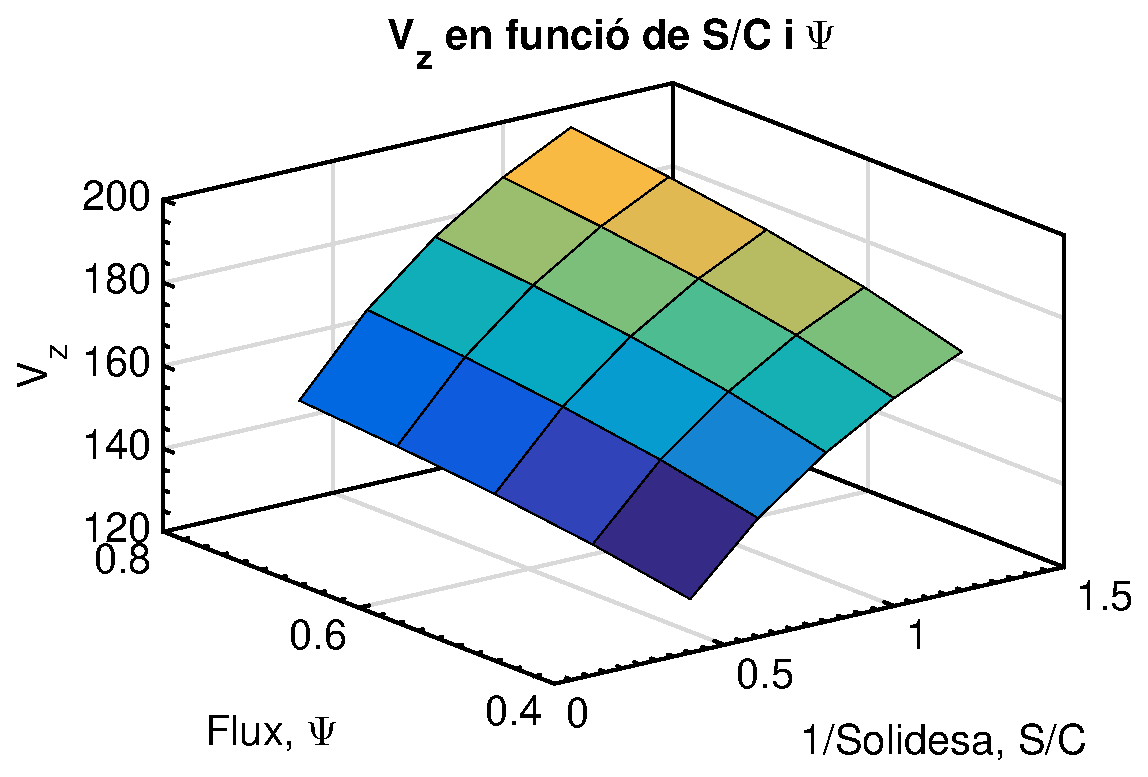
\includegraphics[width=0.8\textwidth]{./code/figures/parametres/Vz}
	\caption{Valors de $V_z$ en funció de $S/C$ i $\Psi$.}
	\label{Vz}
\end{figure}
La velocitat axial haurà d'estar entre els valors de $150m/s$ i $180m/s$. Per sota d'aquests valors el treball aportat per un esglaó es molt baix i per sobre podria donar pas a problemes de combustió. Es verificarà que la velocitat axial estigui entre aquests valors. 
\subsection{Càlcul de la velocitat tangencial en funció de $S/C$ i $\Psi$}
Un cop obtinguda la velocitat axial, calcular la velocitat tangencial es senzill degut a que estan directament relacionades mitjançant el paràmetre de flux. 
\begin{equation}
\Psi=\frac{V_z}{U}
\end{equation}
La velocitat tangencial, o velocitat d'arrossegament, també ha d'estar limitada degut a les càrregues centrífugues que produeix. Per aquesta raó, es verificarà que no sobrepassi el valor de $320m/s$.
\begin{figure}[H]
	\centering
	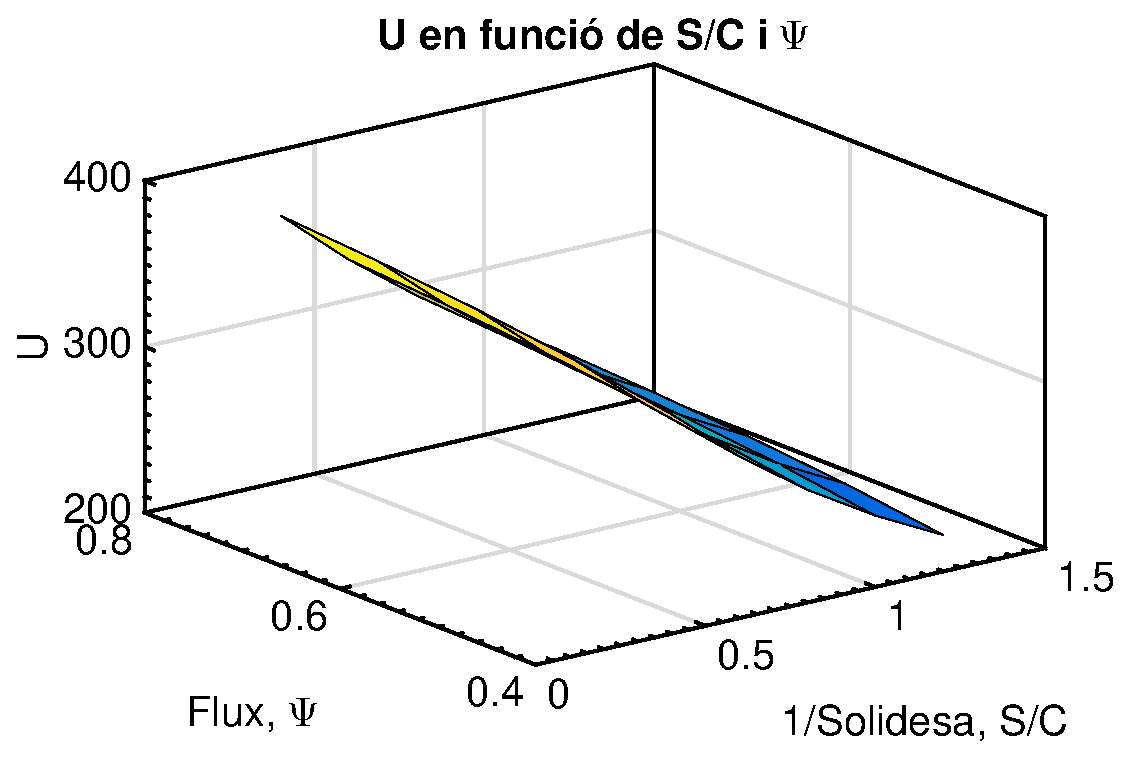
\includegraphics[width=0.8\textwidth]{./code/figures/parametres/U}
	\caption{Valors de $U$ en funció de $S/C$ i $\Psi$.}
	\label{U}
\end{figure}

\subsection{Càlcul del treball de l'esglaó en funció de $S/C$ i $\Psi$}
El treball per esglaó es calcula utilitzant:
\begin{equation}
\tau_{esg}=UV_z(\tan\beta_a-\tan\beta_b)
\end{equation}
\begin{figure}[H]
	\centering
	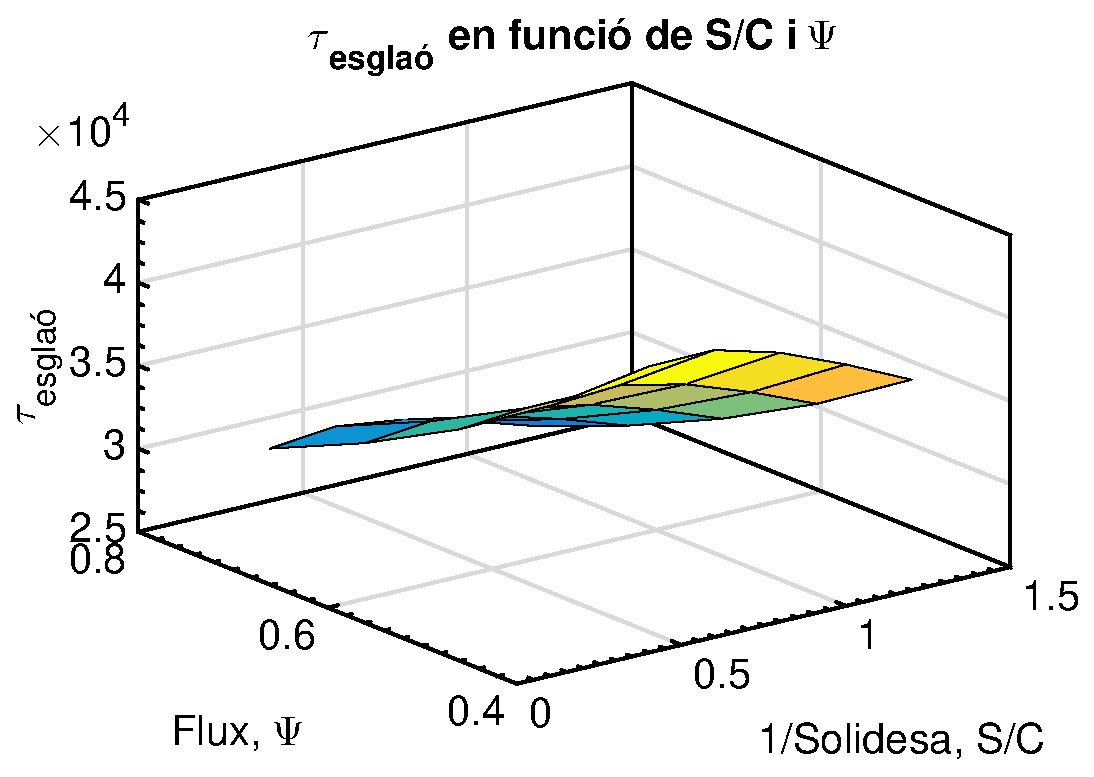
\includegraphics[width=0.8\textwidth]{./code/figures/parametres/TAUesg}
	\caption{Valors de $\tau_{esg}$ en funció de $S/C$ i $\Psi$.}
	\label{TAUesg}
\end{figure}

\subsection{Càlcul de la relació de radis en funció de $S/C$ i $\Psi$}
Es busca calcular al relació entre els radis exterior i interior de l'àlep. Per tal de trobar-la, es necessari realitzar un estudi sobre els esforços centrífugs. Es considerarà que l'àlep te una forma cilíndrica. Com que aquesta suposició no es real, s'haurà d'incorporar el següent factor:
\begin{equation}
\lambda=\frac{\sigma_{real}}{\sigma_{cilindre}}
\end{equation}
El valor de $\lambda$ oscil·la entre $0.6$ y $0.8$. En aquest disseny es prendrà $\lambda=0.7$.
La força centrífuga es pot calcular com: 
\begin{equation}
F_c=\int_{r_i}^{r_e} A(r)\rho\omega^2rdr
\end{equation}
L'esforç a un àlep es: 
\begin{equation}
\sigma=\frac{\rho\omega^2}{A}\int_{r_i}^{r_e} A(r)rdr
\end{equation}
Tenint en compte la consideració ja mencionada d'assimilar l'àlep a un geometria cilíndrica amb àrea constant: 
\begin{equation}
\sigma_{cilindre}=\rho\omega^2\frac{r_e^2-r_i^2}{2}
\end{equation}
Aplicant el factor de correcció $\lambda$:
\begin{equation}
\sigma_{real}=\lambda\rho\omega^2\frac{r_e^2-r_i^2}{2}
\end{equation}
Operant amb els valors coneguts fins ara es pot arribar a l'expressió: 
\begin{equation}
\frac{r_i}{r_e}=\frac{U^2-\frac{\sigma}{2\lambda\rho}}{U^2+\frac{\sigma}{2\lambda\rho}}
\label{rireeq}
\end{equation}
Amb l'objectiu d'incorporar un factor de seguretat: 
\begin{equation}
\sigma=\frac{\sigma_{max}}{4}
\end{equation}
Els valors de $\sigma_{max}$ i de densitat estan definits pel material utilitzat per a construir aquesta primera etapa. Es considera que el material serà un aliatge d'alumini: L-316. Les seves característiques son: 
\begin{equation}
\nonumber \sigma_{max}=39·10^6 kg/m^2
\end{equation}
\begin{equation}
\nonumber \rho=2.8 kg/dm^2
\end{equation}
\begin{figure}[H]
	\centering
	\includegraphics[width=0.8\textwidth]{./code/figures/parametres/rire}
	\caption{Valors de $r_i/r_e$ en funció de $S/C$ i $\Psi$.}
	\label{rire}
\end{figure}

\subsection{Càlcul del radi exterior, radi interior, radi mitjà i altura en funció de $S/C$ i $\Psi$}
Es calcula el radi exterior utilitzant la següent expressió del flux màssic (consum, G) al compressor: 
\begin{equation}
G=2\rho V_z\pi\Big(\frac{r_e^2-r_i^2}{2}\Big)
\end{equation}
Aïllant es pot obtenir: 
\begin{equation}
r_e=\sqrt{\frac{G}{\pi\Big(1-\frac{r_i^2}{r_e^2}\Big)V_z\rho_{at}}}
\end{equation}
Un cop obtingut el valor del radi exterior, el radi interior es pot calcular amb l'expressió \ref{rireeq}. L'altura dels àleps es la diferencia entre el radi exterior i el radi interior: 
\begin{equation}
h=r_e-r_i
\end{equation}
Els valors obtinguts son els següents: 
\begin{figure}[H]
	\centering
	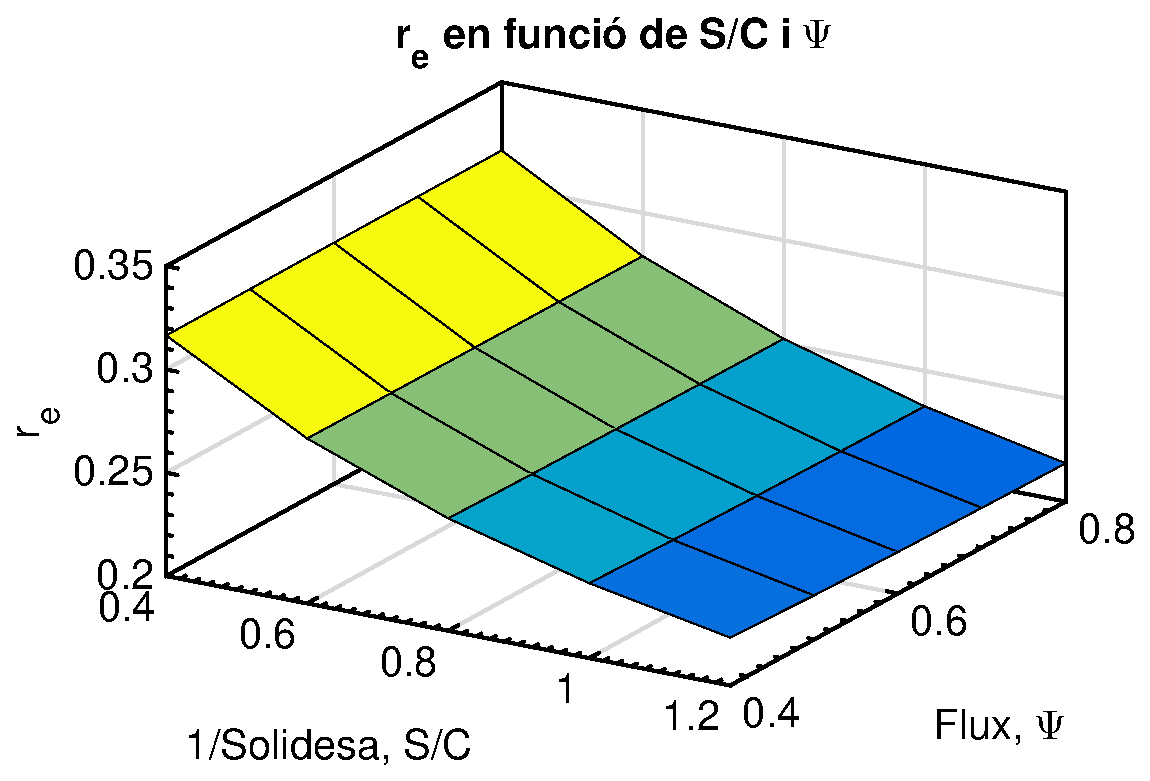
\includegraphics[width=0.8\textwidth]{./code/figures/parametres/re}
	\caption{Valors de $r_e$ en funció de $S/C$ i $\Psi$.}
	\label{re}
\end{figure}


\begin{figure}[H]
	\centering
	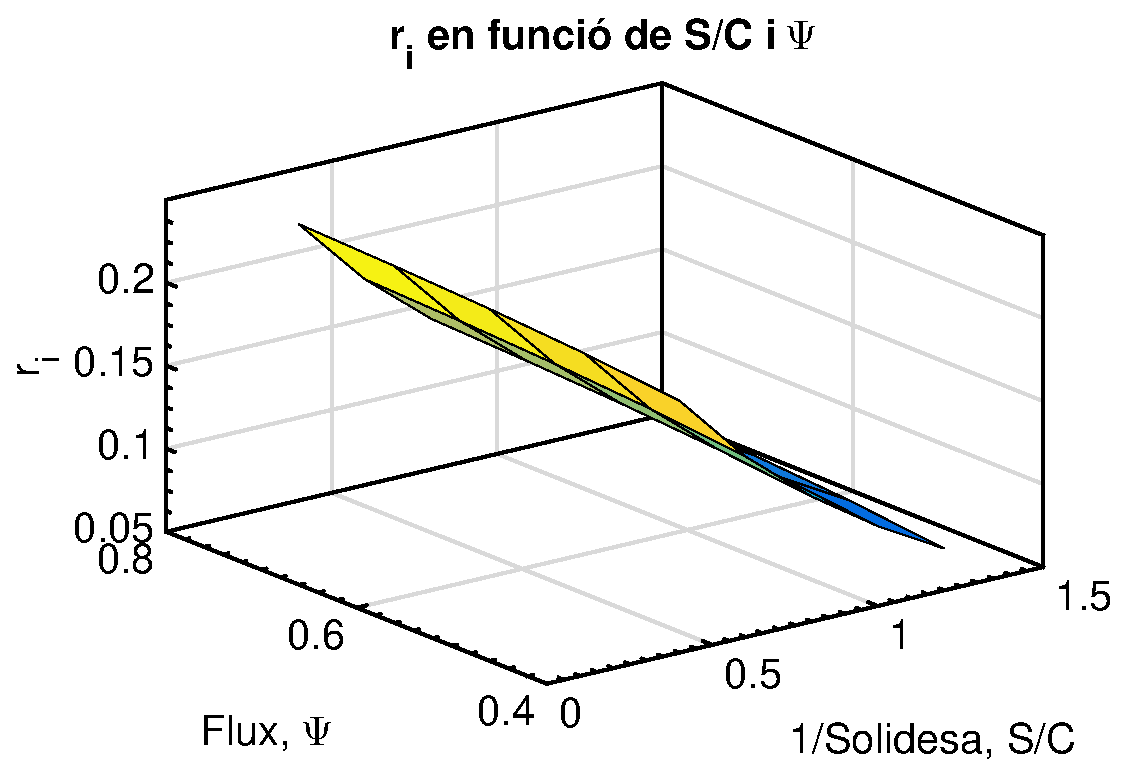
\includegraphics[width=0.8\textwidth]{./code/figures/parametres/ri}
	\caption{Valors de $r_i$ en funció de $S/C$ i $\Psi$.}
	\label{ri}
\end{figure}


\begin{figure}[H]
	\centering
	\includegraphics[width=0.8\textwidth]{./code/figures/parametres/rm}
	\caption{Valors de $r_m$ en funció de $S/C$ i $\Psi$.}
	\label{rm}
\end{figure}

\begin{figure}[H]
	\centering
	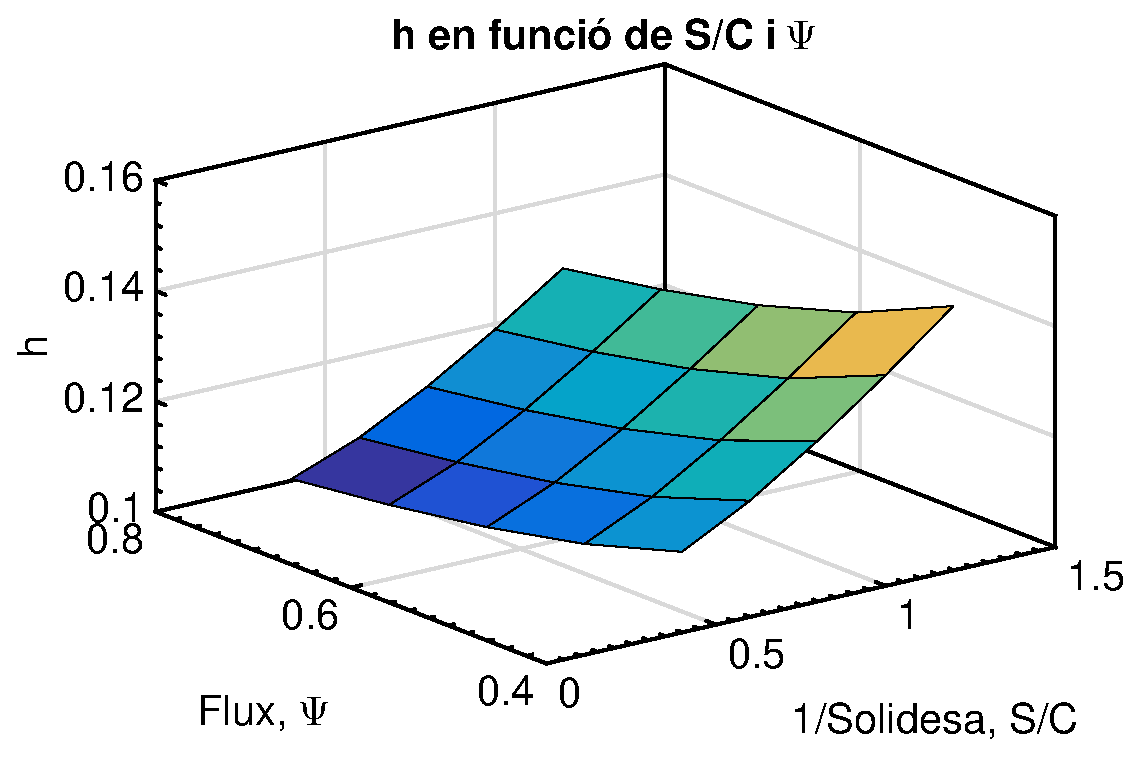
\includegraphics[width=0.8\textwidth]{./code/figures/parametres/h}
	\caption{Valors de $h$ en funció de $S/C$ i $\Psi$.}
	\label{h}
\end{figure}

\subsection{Càlcul de la velocitat de gir en funció de $S/C$ i $\Psi$}
Per últim, es calcula la velocitat de gir del rotor. Aquesta es: 
\begin{equation}
N(rpm)=\frac{60U}{2\pi r_m}
\end{equation}

\begin{figure}[H]
	\centering
	\includegraphics[width=0.8\textwidth]{./code/figures/parametres/RPM}
	\caption{Valors de $N$ en funció de $S/C$ i $\Psi$.}
	\label{RPM}
\end{figure}